\chapter{Interfacing UltraSonic sensors}
\label{ch:ultrasonic}
%------------------------------------------------
\par Defined by the American National Standards Institute, a ultra-sound are sound frequencies greater than 20Khz. They are normal sound waves which humans cannot hear, but some animals can. Humans ears can detect sound of frequencies in the range from 20Hz to 20KHz. Ultra sonic waves behave similar to normal sound waves i.e., they propagate at 340m/s and reflects upon striking a surface. They are widely employed in detection and raging, imaging, under water communication etc.

\begin{figure}
	\centering
	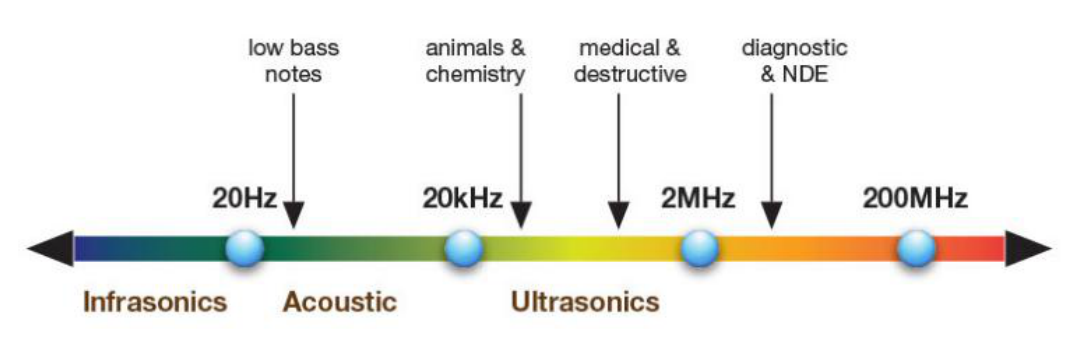
\includegraphics[width=4.3in]{Images/Ultrasonic/spectrum.png}
	\caption{The Ultrasonic Spectrum}
\end{figure}

 The production of ultrasonic waves requires a transmitter that transmit wave pulses, which are then received by a receiver. These two unites are imprinted in a board to be synchronous in achieving the task. The sensor is controlled by digital signals (pulses), produced/controlled by micro controllers or processors. 
%------------------------------------------------

\section{Ultrasonic sensor}
\par There are various series of ultrasonic sensor available. They differ in their functionality on the projects. Few sensors have higher sensitivity, other few have more or less number of connection pins etc. The utility of each sensor is based on the projects they are used. Few sensors can be preferred more that other sensor in a particular project. In this session, we would be detailing about HC-SR04,  one of the commonly used ultrasonic sensors.

\begin{figure}
    \centering
    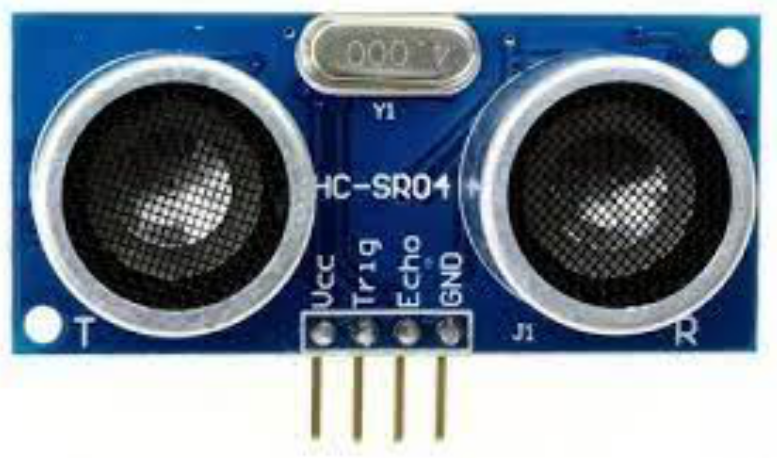
\includegraphics[width=3.5in]{Images/Ultrasonic/board.png}
    \caption{HC-SR04 Ultrasonic Sensor}
	\setfloatalignment{b}
\end{figure}

\section{Detailing HC-SR04 ultrasonic sensor}

\par HC-SR04 is the most commonly used ultrasonic sensor. It is interfaced with Arduino via four pins. The board have a two cylinder like structures with a mesh/net on them. They are the transmitter and receivers made up of crystals of materials such as quartz that vibrate very fast when electricity is passed through them—an effect called “piezoelectricity.” As they vibrate, they manipulate the air around them and the fluids they come in contact with, producing ultrasonic waves. In transmitter the electricity is passed to the crystal to produce waves. In the receiver, the vibrating crystal produce small voltages that are detected and amplified. The cylinder that transmit waves have a small marking “T” at the edge and the receiver have a “R” marking at its edge. To synchronize the activity, the board has and 4Mhz oscillator to act as a timer. This specific board can detect an object if it is between 2-40cm range in front of the sensors.

\begin{figure}
	\centering
	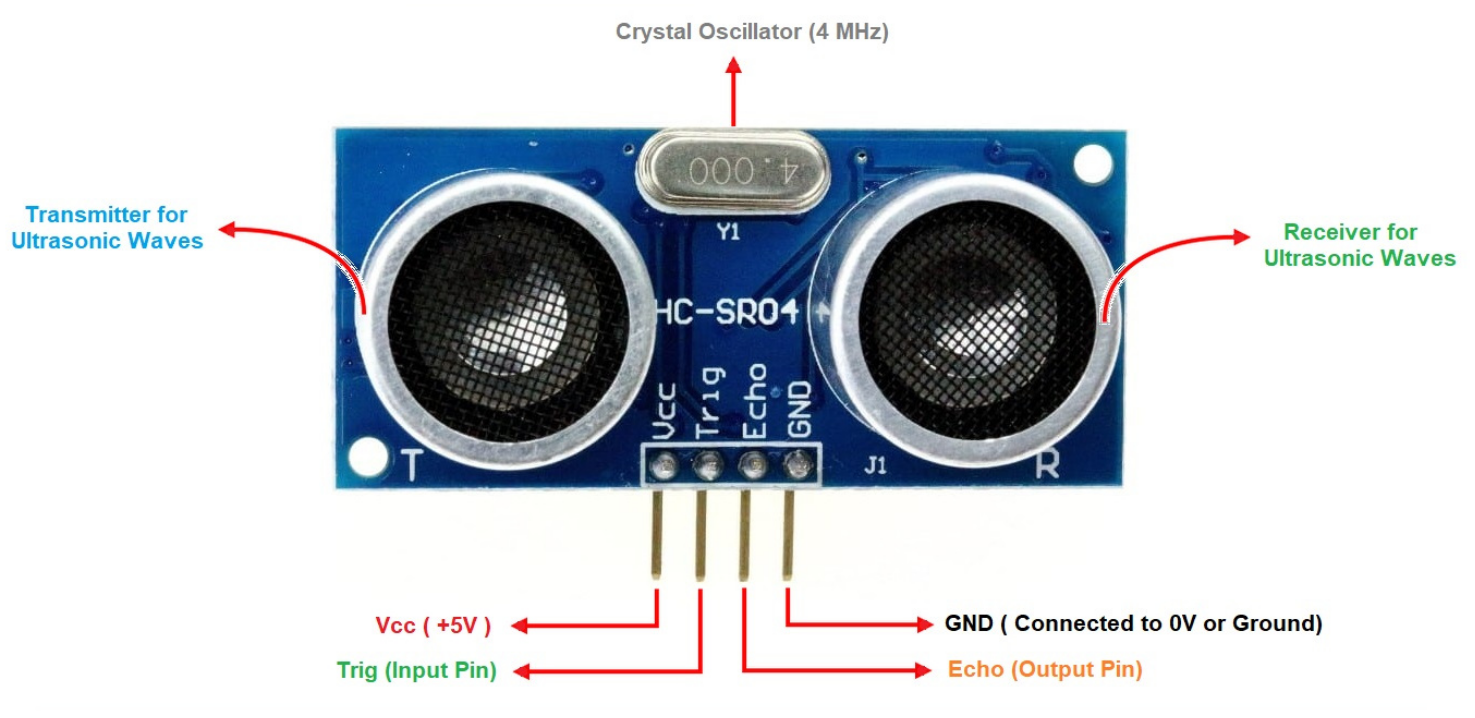
\includegraphics[width=4.3in]{Images/Ultrasonic/pinout.png}
	\caption{HC-SR04 Pinout}
\end{figure}

\section{Pins on HC-SR04}
The board have 4 pins, they are VCC, TRIG, ECHO, GND. To power up the sensor, 5V and GND of Arduino are connected to the VCC and GND pins of the sensor. The TRIG is the input pin, that denote how long should the sensor produce ultrasonic waves. The ECHO is the output pin that denotes how long have we waited to receive the ultrasonic wave. Keep in mind that the input of the sensor will be connected to the output pin of Arduino and the output pin of sensor will be interfaced as input pin for Arduino. In short, the signal travels from sensor to Arduino in ECHO pin and from Arduino to sensor in TRIG pin.

\section{Working of HC-SR04 sensor}


\begin{figure}
    \centering
    \subfloat[Transmission]{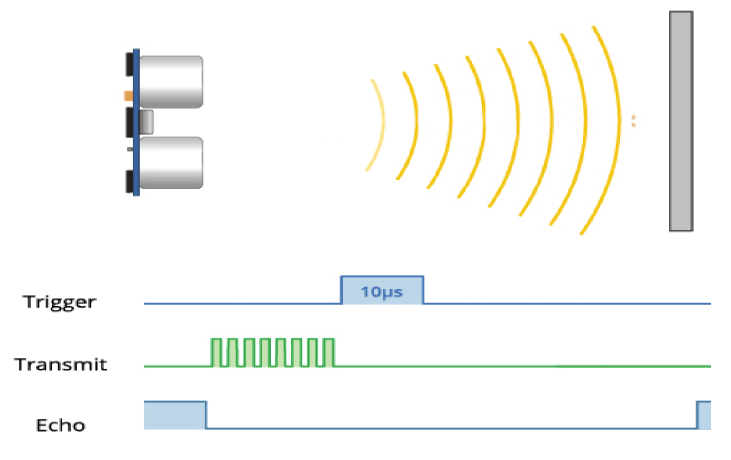
\includegraphics[width=2in]{Images/Ultrasonic/transmission.png}}\qquad
    \subfloat[Receiving]{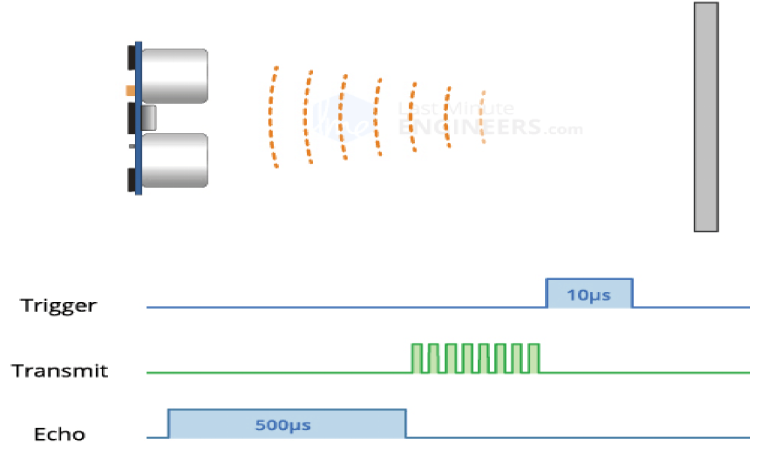
\includegraphics[width=2in]{Images/Ultrasonic/receiving.png}}
    \caption[Ultrasonic - Working]{Ultrasonic waves bounces from surface}
\end{figure}
\vspace{0.5cm}

Initially we would put TRIG pin high for about 10 micro seconds. The sensor, upon receiving this signal, produce eight 40KHz pulses automatically. After producing short pulse burst, it would start the timer and pulls the ECHO pins to a high signal. It would then wait for the transmitted signal to reach back to the sensor. Upon receiving the first wave, it pulls the ECHO pin to low. We would record the time the ECHO pin remained high to calculate the distance between the sensor and the object.

\section{Calculation of the distance}
We know that 
\begin{align*}
    speed &= \frac{distance}{time}
\end{align*}
Or,
\begin{align*}
    distance &= speed * time
\end{align*}  
We have,
\par Speed of sound = 340m/s
\par Time can be fetched from the ultrasonic sensors.

\vspace{0.5cm}
\par Do note that the speed is in m/s and the time we receive is in µs. Lets formulate a formula to convert the units so that the distance can be measured in centi-meters (cm).

\par Let ‘ t ’ denote the time we get from sensor in µs. Keep in mind that this time it the time taken by the waves to travel from sensors to the object and back to the sensors. In short, they have covered the distance twice. So the time required by the wave to travel from sensors to object is t/2 µs. Lets substitute the values in the formula

\begin{align*}
    distance &= 340 m/s * \frac{t}{2} \hspace{0.1cm} \mu s \\
    distance &= 340 * \frac{t}{2} \hspace{0.1cm} \frac{m \mu s}{s} \\
    distance &= 170t\hspace{0.1cm} \mu m \\
    distance &= 170t * 10^{-6} \hspace{0.1cm} m \\
    distance &= 170t * 10^{-4} \hspace{0.1cm} cm \\
    \vspace{0.3cm}\\
    \textbf{distance} &= \textbf{0.017t} \hspace{0.1cm} \textbf{cm}
\end{align*}


\section{\textbf{Code example 1}}
\par Objective : To print the distance of a object from sensor in serial monitor.

\begin{lstlisting}[style=CStyle]
int TRIG = 10;           //trigger pin of sensor
int ECHO =  9;           //echo pin of sensor
long duration;           //to store the time (micro seconds)
float distance;          //to store the distance (cm)

void setup(){
    pinMode(TRIG,OUTPUT);     //TRIG as output of Arduino
    pinMode(ECHO,INPUT);      //ECHO as input of Arduino
    Serial.begin(9600);       //Baud rate
}

void loop(){
    //wait for some time to clear the ultrasonic
    //waves if present in environment
    digitalWrite(TRIG,LOW);
    delayMicroseconds(2);
    
    //create ultrasonic burst
    digitalWrite(TRIG,HIGH);
    delayMicroseconds(10);
    degitalWrite(TRIG,LOW);
    
    //record the duration ECHO pin stood HIGH
    duration = pulseIn(ECHO,HIGH);
    
    //calculate the distance
    distance = 0.017 * duration;
    
    //print the distance
    Serial.print("The object is at ");
    Serial.print(distance);
    Serial.println(" cm");
    
    //Slow down the code so that serial monitor
    //does not flood with characters
    delay(1000);					
}
\end{lstlisting}

\begin{figure}[h!]	
	\centering
	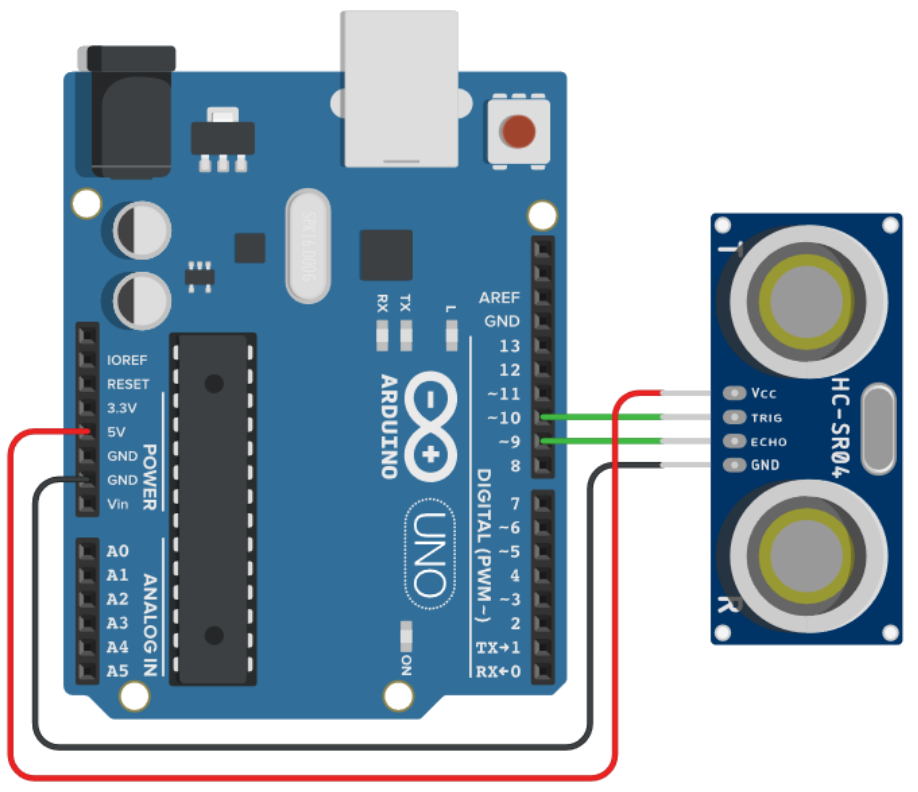
\includegraphics[width=4.3in]{Images/Ultrasonic/circuit1.png}
    \caption{Ultrasonic Sensor with Arduino}
\end{figure}

It is always advised to to wait for at least 2µs to clear the already existing ultrasonic wave in the environment. Try moving the hand in front of sensor to see varying distances. What would happen if we kept our hand on the sensor ( i.e. 0cm distance)? Why does it show high value instead of printing zero? Keep in mind that the receiver need to detect some ultrasonic waves to pull the ECHO pin down.

\section{Object avoider-bot}

Let us now try to create a bot that can avoid the objects in front of it and keep travelling. There are various models of such bot available. In this session we would be making use of two ultrasonic sensors and a bot (with chassis, motor, motor driver, wheel) to construct an object avoider bot. Get an peek into the chapter “Motor Driver” to know various part of constructing a bot. We would be making use of bot build in the chapter “Motor Driver” to construct our object avoider bot.

\begin{figure}
    \centering
    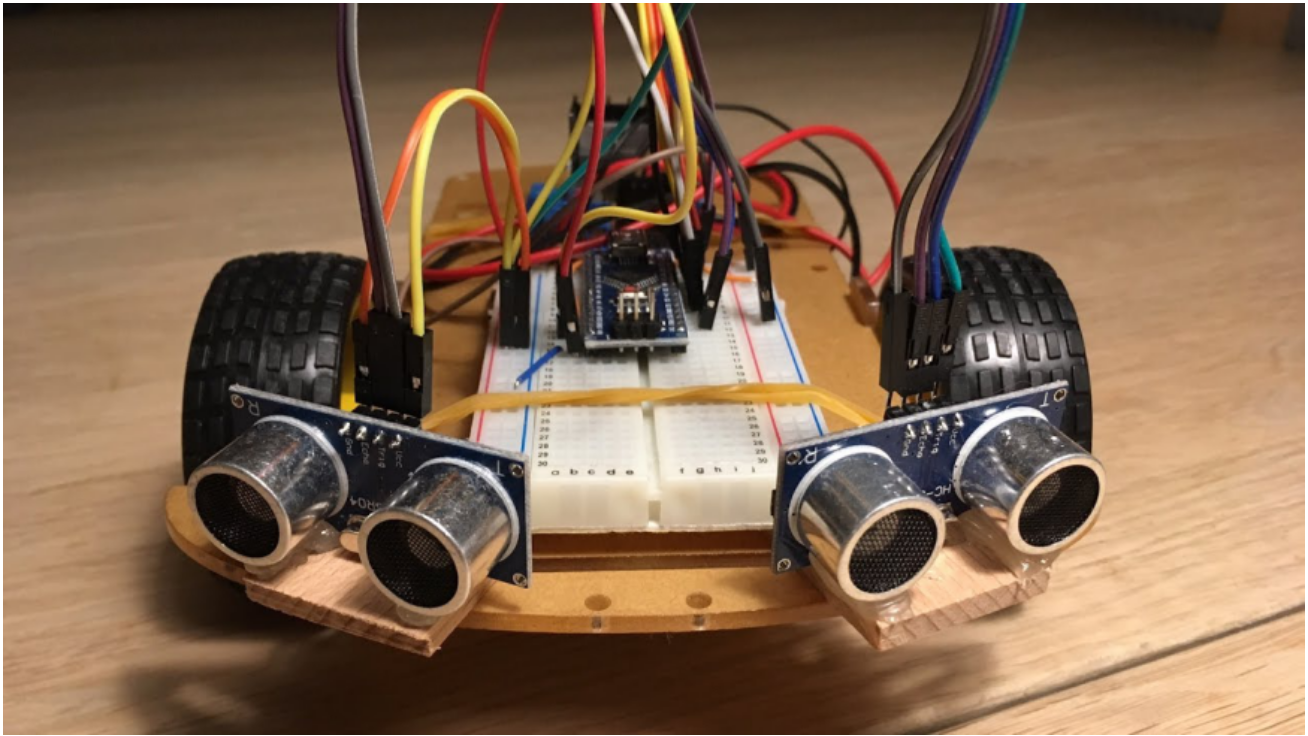
\includegraphics[width=4in]{Images/Ultrasonic/nano_obj_avoider1.png}
    \caption[Obstacle Avoider Bot]{Obstacle Avoider Bot using Arduino Nano}
\end{figure}

We will be programming the bot to avoid the obstacle if it comes less than 10cm in front of the bot. The table \ref{fig: obj_avoider_motion} summarizes our flow.

\begin{figure}
    \centering
    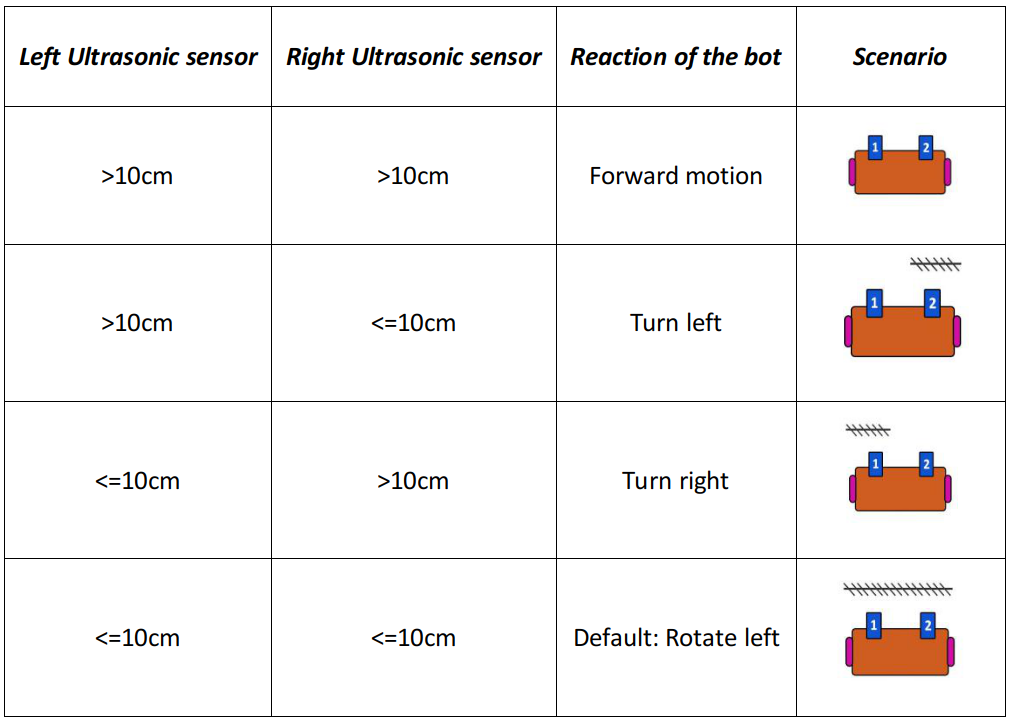
\includegraphics[width=4in]{Tables/Ultrasonic/obj_avoider_movement.png}
    \caption{Obstacle Avoider Motion}
    \label{fig: obj_avoider_motion}
\end{figure}


% \begin{table}[h!]
%     \begin{tabular}{|c|c|c|c|}
%     \hline
%     \textbf{Left Ultrasonic Sensor}& \textbf{Right Ultrasonic sensor} & 
%     \textbf{Reaction of the bot} &
%     \textbf{Scenario} \\
%     \hline
%     >10cm & >10cm & Forward motion &
%     \parbox[c]{6em}{ 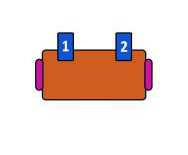
\includegraphics[width=0.7\textwidth,height=20mm]{Chapters/images/ultraSonic_objAvoider_straight.png}} \TBstrut \\
%     \hline
%     >10cm & <=10cm & Turn left &
%     \parbox[c]{6em}{    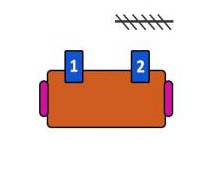
\includegraphics[width=0.7\textwidth,height=20mm]{Chapters/images/ultraSonic_objAvoider_left.png.png}} \TBstrut \\
%     \hline
%     <=10cm & >10cm & Turn right &
%     \parbox[c]{6em}{    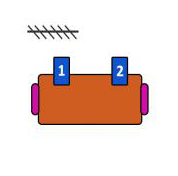
\includegraphics[width=0.7\textwidth,height=20mm]{Chapters/images/ultraSonic_objAvoider_right.png}} \TBstrut \\
%     \hline
%     <=10cm & <=10cm & Default: Rotate left &
%     \parbox[c]{6em}{    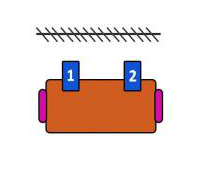
\includegraphics[width=0.7\textwidth,height=20mm]{Chapters/images/ultraSonic_objAvoider_rotate.png}} \TBstrut \\
%     \hline
%     \end{tabular}
% \end{table}
\vspace{2cm}
Here we have listed all sort of possible combinations with 2 IR sensors. Now lets implement them in our bot. Take a quick peek at the section \ref{section:bot_interface} where we have programmed a small bot. Lets add the additional ultrasonic sensors to them to complete our obstacle avoider.

\begin{figure}
    \centering
    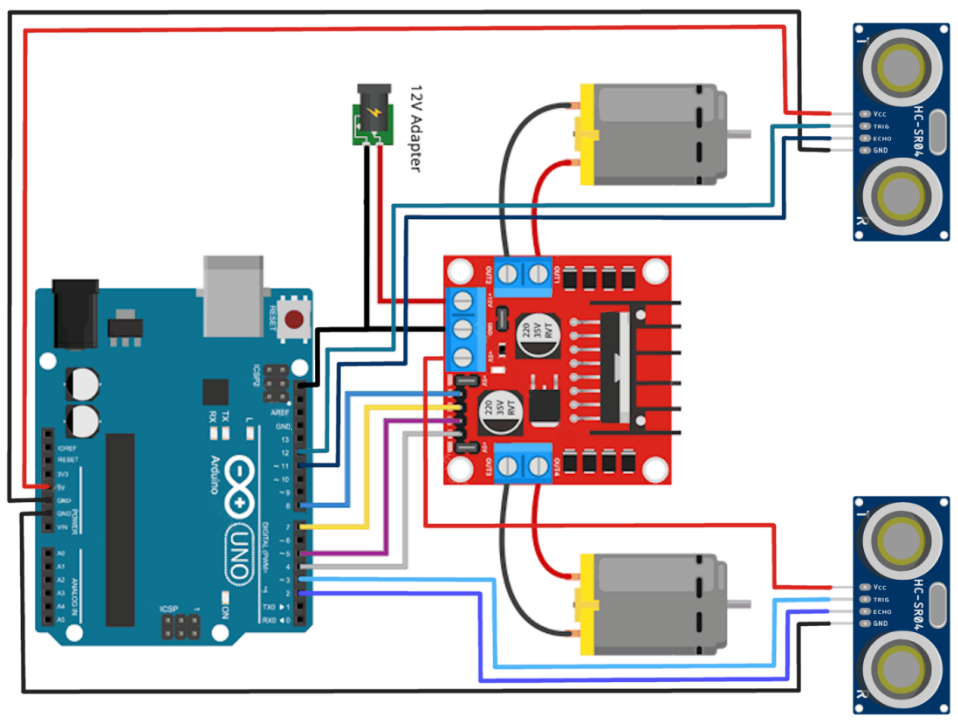
\includegraphics{Images/Ultrasonic/obj_avoider_ckt.png}
     \caption{Obstacle Avoider Circuit}
	\setfloatalignment{b}
\end{figure}

\par Lets simplify the connections. First connect motors to motor driver. Now lets interface motor driver with Arduino Uno. Connect the pins input1, input2, input3, input4 of motor drive to Arduino pins 8, 7, 5 and 4 receptively. The left ultrasonic sensor (top) have its TRIG and ECHO pins connected to 12 and 11 pins of Arduino. Connect its VCC and GND to Arduino 5V and GND respectively. The right ultrasonic sensor (bottom) have its TRIG and ECHO pins connected to 3 and 2 pins of Arduino. Connect its VCC to 5V pin of motor driver and GND to GND pin of Arduino. Each ultrasonic sensor needs separate 5V line. If there are no other 5V source, then you can set any unused pin of Arduino to HIGH and extract 5V from that pin. Finally connect the 12V power line to 12V pin of motor driver and GND pin of motor driver to GND of Arduino and the negative terminal of the 12V source. Power the Arduino using USB cable. With that we have completed the circuits. Now lets build the code.

\pagebreak
\begin{lstlisting}[style=CStyle]
int m1 = 8, m2 = 7;             //left  motor pins
int m3 = 5, m4 = 4;             //right motor pins

int trig_L = 12, echo_L = 11;   //left ultrasonic sensors
int trig_R = 3, echo_R = 2;     //right ultrasonic sensors

float distance_L, distance_R;   //to store each distances
long duration;                  //to store time temporarily
float obj_dist = 10.0;          //threshold distance

void setup(){
    //set motor pins as output for Arduino.
    pinMode(m1,OUTPUT); pinMode(m2,OUTPUT);
    pinMode(m3,OUTPUT); pinMode(m4,OUTPUT);
    
    //set TRIG pins as OUTPUT and ECHO pins as INPUT
    pinMode(trig_L,OUTPUT); pinMode(echo_L,INPUT);
    pinMode(trig_R,OUTPUT); pinMode(echo_R, INPUT);
    
    Serial.begin(9600);
}

//A function to control motor movement
void turn_motor(int input1, int input2, char dir){
    if( dir == 'F'){
        //clockwise rotation
        digitalWrite(input1,HIGH);
        digitalWrite(input2,LOW);
    }
    else if( dir == 'B'){
        //anti-clockwise rotation
        digitalWrite(input1,LOW);
        digitalWrite(input2,HIGH);
    }
    else if( dir == 'S'){
        //no rotation
        digitalWrite(input1,LOW);
        digitalWrite(input2,LOW);
    }
}

void loop(){
    
    // reading value from left sensors
    digitalWrite(trig_L,LOW);
    delayMicroseconds(2);
    digitalWrite(trig_L,HIGH);
    delayMicroseconds(10);
    degitalWrite(trig_L,LOW);
    duration = pulseIn(echo_L,HIGH);
    distance_L = 0.017 * duration;
    
    // reading value from right sensors
    digitalWrite(trig_R,LOW);
    delayMicroseconds(2);
    digitalWrite(trig_R,HIGH);
    delayMicroseconds(10);
    degitalWrite(trig_R,LOW);
    duration = pulseIn(echo_R,HIGH);
    distance_R = 0.017 * duration;
    
    if( distance_L > obj_dist && distance_R > obj_dist ){
        //forward motion
        turn_motor(m1, m2, 'F');  //left  wheel : clockwise
        turn_motor(m3, m4, 'F');  //right wheel : clockwise
        Serial.println("Bot moving forward");
    }
    else if( distance_L > obj_dist && distance_R <= obj_dist ){
        //left motion
        turn_motor(m1, m2, 'S');  //left  wheel : stop
        turn_motor(m3, m4, 'F');  //right wheel : clockwise
        Serial.println("Bot moving left");
    }
    else if( distance_L <= obj_dist && distance_R > obj_dist ){
        //right motion
        turn_motor(m1, m2, 'F');  //left  wheel : clockwise
        turn_motor(m3, m4, 'S');  //right wheel : stop
        Serial.println("Bot moving right");
    }
    else if( distance_L <= obj_dist && distance_R <= obj_dist ){
        //by default, rotate left
        turn_motor(m1, m2, 'B');  //left  wheel : anti-clockwise
        turn_motor(m3, m4, 'F');  //right wheel : clockwise
        Serial.println("Bot rotating left");
        delay(1000); 	//let the bot rotate a bit!!
    }
    delay(100);
}
\end{lstlisting}

\par Try out the same bot by controlling the speeds of wheels. Setup a dummy cardboard maze puzzle and try to solve the puzzle using the bot. You might need to make use of additional concepts to effectively navigates through the edges of walls. You could also rebuild the object avoider bot using single ultrasonic sensor and a servo motor. Put your thoughts and imaginations to get new ideas and solve new challenges.

\begin{figure}
    \centering
    \subfloat[Maze]{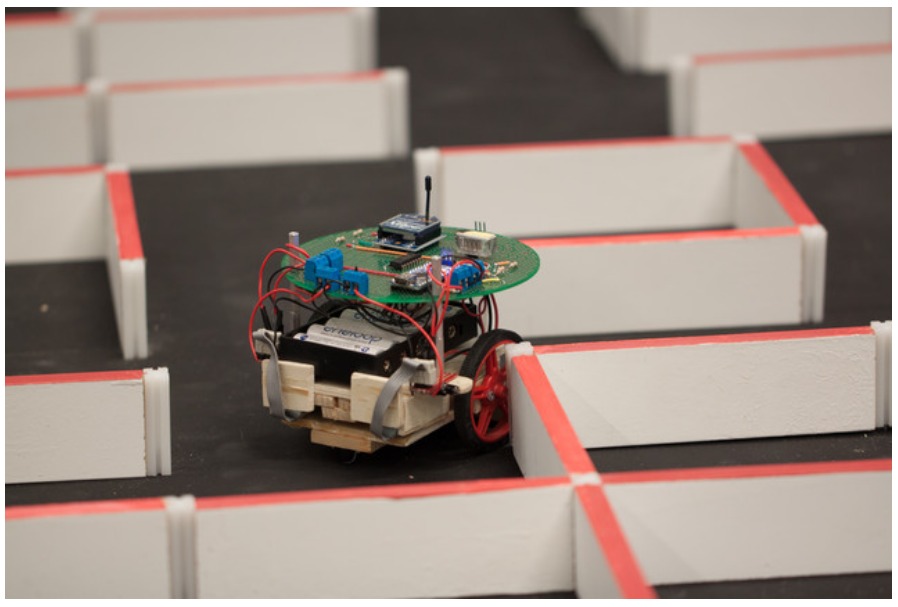
\includegraphics[width=2in]{Images/Ultrasonic/carboard_maze.png}}\quad
    \subfloat[Object Avoider]{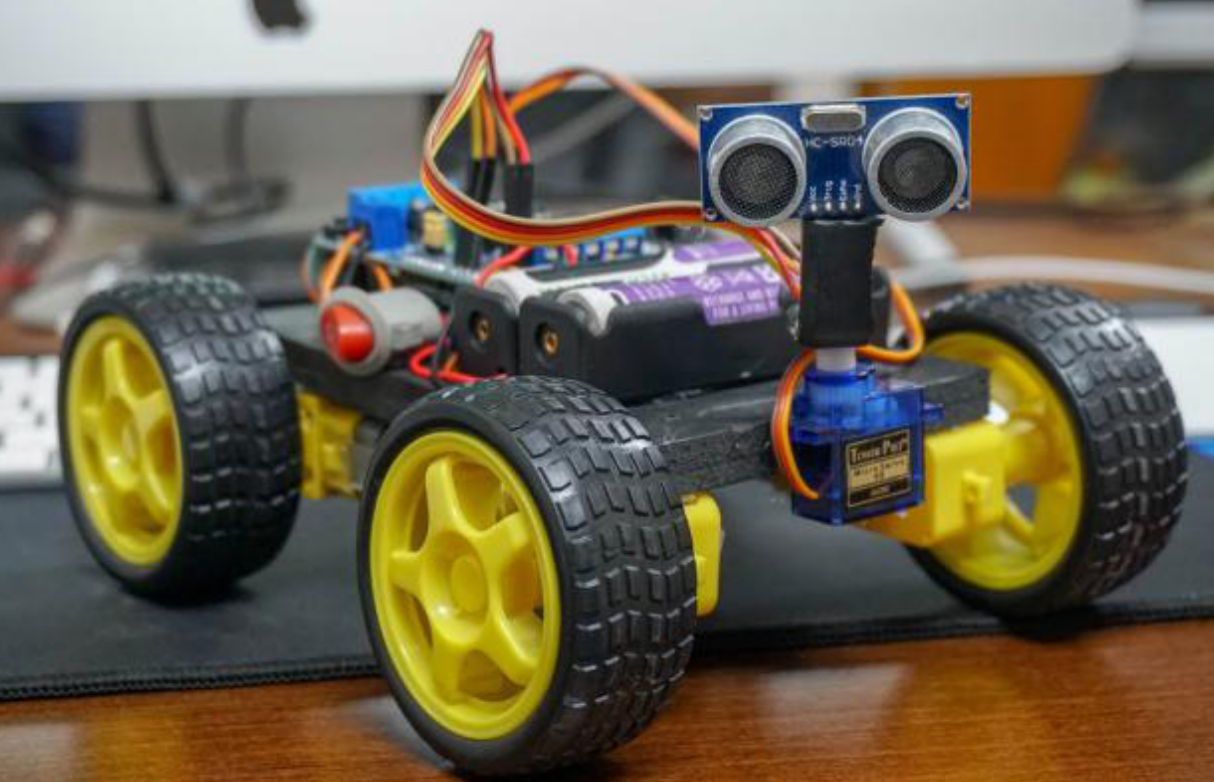
\includegraphics[width=2in]{Images/Ultrasonic/obj_avoider_single.png}}
    \caption[Object Avoider Bots]{Different models and usage of object avoider}
\end{figure}